\renewcommand{\theequation}{\theenumi}
\begin{enumerate}[label=\arabic*.,ref=\thesection.\theenumi]
\numberwithin{equation}{enumi}

\item A bus starting from rest moves with a uniform acceleration of $0.1 m s^{-2}$
for 2 minutes. Find 

\begin{enumerate} 
\item the speed acquired, 
\item the distance travelled.
\end{enumerate}

\item A train is travelling at a speed of $90 km h^{-1}$
. Brakes are applied . Find
so as to produce a uniform acceleration of $- 0.5 m s^{-2}$
how far the train will go before it is brought to rest.
\item  A trolley, while going down an inclined plane, has an acceleration of $2 cm s^{-2}$
. What will
be its velocity $3 s$ after the start? . What
\item  A racing car has a uniform acceleration of $4 m s^{-2}$
distance will it cover in $10 s$ after start?
\item  A stone is thrown in a vertically upward direction with a velocity of $5 m s^{-1}$
. If the acceleration of the
stone during its motion is $10 m s^{-2}$ in the downward direction, what will be the height attained by the stone and how much time will it take to reach there?

\item An athlete completes one round of a circular track of diameter 200 m in 40 s. What will be the distance covered and the displacement at the end of 2 minutes 20 s?
\item  Joseph jogs from one end A to the other end B of a straight 300 m road in 2 minutes 30 seconds and then turns around
and jogs 100 m back to point C in another 1 minute. What are Joseph's average speeds and velocities in jogging 

\begin{enumerate} 
\item from A to B and 
\item from A to C?
\end{enumerate}

\item  Abdul, while driving to school, computes the average speed for his trip to be 20 $km h^{-1}$
. On his return trip along the same
route, there is less traffic and the average speed is 30 $km h^{-1}$
. What is the average speed for Abdul's trip?
\item  A motorboat starting from rest on a lake accelerates in a straight line at a constant rate of 3.0 $m s^{-2}$
for 8.0 s. How far does the boat travel during this time? 
\item  A driver of a car travelling at 52 $km h^{-1}$
applies the brakes and in another car applies
accelerates uniformly in the opposite direction. The car stops in 5 s. Another driver going at 3 $km h^{-1}$
his brakes slowly and stops in 10 s. On the same graph paper, plot the speed versus time graphs for the two cars. Which of the two cars travelled farther after the brakes were applied?

\item A ball is gently dropped from a height of 20 m. If its velocity increases uniformly at the rate of 10 $m s^{-2}$
, with what velocity
will it strike the ground? After what time will it strike the ground?

\item An artificial satellite is moving in a circular orbit of radius 42250 $km$. Calculate its speed if it takes 24 hours to revolve around the earth.
\item From a rifle of mass 4 kg, a bullet of mass 50 g is fired with an initial velocity of 35 $m s^{-1}$
.
Calculate the initial recoil velocity of the rifle.
\item Two objects of masses 100 g and 200 g are moving along the same line and direction with velocities of 2 $m s^{-1}$ and 1 $m s^{-1}$ , respectively. 
They collide and after the collision, the first object moves at a velocity of 1.67 $m s^{-1}$ 
. Determine the velocity of the second object.

\item A truck starts from rest and rolls down a hill with a constant acceleration. It travels a distance of 400 m in 20 s. Find its acceleration. Find the force acting on it if its mass is 7 tonnes (Hint: 1 tonne = 1000 kg.)
\item  A stone of 1 kg is thrown with a velocity of 20 $m s^{-1}$ across
the frozen surface of a lake and comes to rest after travelling a distance of 50 m. What is the force of friction between the stone and the ice?
\item  A 8000 kg engine pulls a train of 5 wagons, each of 2000 kg, along a horizontal track. If the engine exerts a force of 40000 N and the track offers a friction force of 5000 N, then calculate: 
\begin{enumerate} 
\item the net accelerating force and 
\item the acceleration of the train.
\end{enumerate}
\item  An automobile vehicle has a mass of 1500 kg. What must be the force between the vehicle and road if the vehicle is to
be stopped with a negative acceleration of 1.7 $m s^{-2}$ 
\item  Using a horizontal force of 200 N, we intend to move a wooden cabinet across a floor at a constant velocity. What is the friction force that will be exerted on the cabinet?
\item  Two objects, each of mass 1.5 kg, are moving in the same straight line but in opposite directions. The velocity of each object is 2.5 $m s^{-1}$
before the collision during which they stick together. What will be the velocity of the combined object after collision?
\item A hockey ball of mass 200 g travelling at 10 $m s^{-1}$ is struck by
a hockey stick so as to return it along its original path with a velocity at 5 $m s^{-1}$
momentum occurred in the motion of the hockey ball by the force applied by the hockey stick.
\item  A bullet of mass 10 g travelling horizontally with a velocity of 150 $m s^{-1}$
strikes a stationary wooden block and comes to rest in 0.03 s. Calculate the distance of penetration of the bullet into the block. Also calculate the magnitude of the force exerted by the wooden block on the bullet.
\item  An object of mass 1 kg travelling in a straight line with a velocity of 10 $m s^{-1}$
collides with, and sticks to, a stationary wooden block of mass 5 kg. Then they both move off together in the same straight line. Calculate the total momentum just before the impact and just after the impact. Also, calculate the velocity of the combined object.
\item  An object of mass 100 kg is accelerated uniformly from a velocity of 5 $m s^{-1}$
to 8 $m s^{-1}$ in 6 s. Calculate the initial and final
momentum of the object. Also, find the magnitude of the force exerted on the object.
\item  How much momentum will a dumb-bell of mass 10 kg transfer to the floor if it falls from a height of 80 cm? Take its downward acceleration to be 10 $m s^{-2}$. Calculate the magnitude of change of

\item Two persons manage to push a motorcar of mass 1200 kg at a uniform velocity along a level road. The same motorcar can be pushed by three persons to produce an acceleration of 0.2 $m s^{-2}$
. With what force does each person push the motorcar? (Assume that all persons push the motorcar with the same muscular effort.)
\item  A hammer of mass 500 g, moving at 50 $m s^{-1}$ , strikes a nail.
The nail stops the hammer in a very short time of 0.01 s. What is the force of the nail on the hammer?
\item  A motorcar of mass 1200 kg is moving along a straight line with a uniform velocity of 90 km/h. Its velocity is slowed down to 18 km/h in 4 s by an unbalanced external force. Calculate the acceleration and change in momentum. Also calculate the magnitude of the force required.
\item What is the magnitude of the gravitational force between the earth and a 1 kg object on its surface? (Mass of the earth is 6 $\times$ 1024 kg and radius of the earth is 6.4 $\times$ 106 m.)
\item A ball is thrown vertically upwards with a velocity of 49 m/s. Calculate

\begin{enumerate} 
\item  the maximum height to which it rises, 
\item the total time it takes to return to the surface of the earth.
\end{enumerate}

\item  A stone is released from the top of a tower of height 19.6 m. Calculate its final velocity just before touching the ground.
\item  A stone is thrown vertically upward with an initial velocity of 40 m/s. Taking g = 10 $ms^{-2}$
, find the maximum height reached
by the stone. What is the net displacement and the total distance covered by the stone?
\item  Calculate the force of gravitation between the earth and the Sun, given that the mass of the earth = 6 $\times 10^{24}$
kg and of the
Sun = 2 $\times 10^{30}$ kg. The average distance between the two is 1.5 $\times 10^{11}$
m.
\item  A stone is allowed to fall from the top of a tower 100 m high and at the same time another stone is projected vertically upwards from the ground with a velocity of 25 m/s. Calculate when and where the two stones will meet.
\item  A ball thrown up vertically returns to the thrower after 6 s. Find
\begin{enumerate} 
\item the velocity with which it was thrown up, 
\item the maximum height it reaches, and 
\item  its position after 4 s.
\end{enumerate}

\item The volume of 50 g of a substance is 20 $cm^3$ 
. If the density of water is 1 $g cm^{-3}$, will the substance float or sink? 
\item  The volume of a 500 g sealed packet is 350 $cm^3$
Will the packet float or sink in water if the density of water is 1 $g cm^{-3}$ ? What will be the mass of the water displaced by this packet?
\item Certain force acting on a 20 kg mass changes its velocity from 5 $m s^{-1}$
to 2 $m s^{-1}$. Calculate the work done by the force.
\item A certain household has consumed 250 units of energy during a month. How much energy is this in joules?
\item  An object of mass 40 kg is raised to a height of 5 m above the ground. What is its potential energy? If the object is allowed to fall, find its kinetic energy when it is half-way down.
\item An electric heater is rated 1500 W. How much energy does it use in 10 hours?
\item Calculate the work required to be done to stop a car of 1500 kg moving at a velocity of 60 km/h?
\item Find the energy in kW h consumed in 10 hours by four devices of power 500 W each.
\item An echo is heard in 3 s. What is the distance of the reflecting surface from the source, given that the speed of sound is 342 $m s^{-1}$
?  
\item A submarine emits a sonar pulse, which returns from an underwater cliff in 1.02 s. If the speed of sound in salt water is 1531 m/s, how far away is the cliff?
\item A person has a hearing range from 20 Hz to 20 kHz. What are the typical wavelengths of sound waves in air corresponding to these two frequencies? Take the speed of sound in air as 344 $m s^{-1}$
.
\item Two children are at opposite ends of an aluminium rod. One strikes the end of the rod with a stone. Find the ratio of times taken by the sound wave in air and in aluminium to reach the second child.
\item  The frequency of a source of sound is 100 Hz. How many times does it vibrate in a minute?
\item A stone is dropped from the top of a tower 500 m high into a pond of water at the base of the tower. When is the splash heard at the top? Given, g = 10 $m s^{-2}$
and speed of sound = 340 $m s^{-1}$ . 
\item  A sound wave travels at a speed of 339 $m s^{-1}$ 174 . If its
wavelength is 1.5 cm, what is the frequency of the wave? Will it be audible?
\item A sonar device on a submarine sends out a signal and receives an echo 5 s later. Calculate the speed of sound in water if the distance of the object from the submarine is 3625 m.
\item An object 5 cm in length is held 25 cm away from a converging lens of focal length 10 cm. Draw the ray diagram and find the position, size and the nature of the image formed.
\item  A concave lens of focal length 15 cm forms an image 10 cm from the lens. How far is the object placed from the lens? Draw the ray diagram.
\item  An object is placed at a distance of 10 cm from a convex mirror of focal length 15 cm. Find the position and nature of the image.
\item  The magnification produced by a plane mirror is +1. What does this mean? 
\item  An object 5.0 cm in length is placed at a distance of 20 cm in front of a convex mirror of radius of curvature 30 cm. Find the position of the image, its nature and size.
\item  An object of size 7.0 cm is placed at 27 cm in front of a concave mirror of focal length 18 cm. At what distance from the mirror should a screen be placed, so that a sharp focussed image can be obtained? Find the size and the nature of the image.
\item  Find the focal length of a lens of power - 2.0 D. What type of lens is this? 
\item  A doctor has prescribed a corrective lens of power +1.5 D. Find the focal length of the lens. Is the prescribed lens diverging or converging?
\item  Judge the equivalent resistance when the following are connected in parallel - 
\begin{enumerate} \item 1 $\ohm $ and $10^6 \ohm $, \item1 $\ohm $ and $10^3 \ohm$, and $10^6 \ohm$.\end{enumerate}
\item An electric lamp of 100 $\ohm$, a toaster of resistance 50 $\ohm$, and a water filter of resistance 500 $\ohm $ are connected in parallel to a 220 V source. What is the resistance of an electric iron connected to the same source that takes as much current as all three appliances, and what is the current through it?
\item  How can three resistors of resistances 2 $\ohm$, 3 $\ohm$, and 6 $\ohm$ be connected to give a total resistance of
 \begin{enumerate} \item 4 $\ohm$, \item 1 $\ohm$ \end{enumerate}?
\item What is 
\begin{enumerate} \item the highest, \item the lowest total resistance 
\end{enumerate}
that can be secured by combinations of four coils of resistance 4 $\ohm$, 8 $\ohm$, 12 $\ohm$, 24 $\ohm$?
\item  A piece of wire of resistance R is cut into five equal parts. These parts are then connected in parallel. If the equivalent resistance of this combination is R', then the ratio R/R' is -
%\begin{enumerate} \item 1/25 R \item 1/5 \item IR2 \item  5 \item  VI \item  25
%\end{enumerate}
\item  An electric bulb is rated 220 V and 100 W. When it is operated on 110 V, the power consumed will be - 
\item  Two conducting wires of the same material and of equal lengths and equal diameters are first connected in series and then parallel in a circuit across the same potential difference. The ratio of heat produced in series and parallel combinations would be -
\item  A copper wire has diameter 0.5 mm and resistivity of 1.6 $\times 10^{-8} \ohm$ m. What will be
the length of this wire to make its resistance 10 $\ohm$? How much does the resistance change if the diameter is doubled?
\item  The values of current I (amperes)  flowing in a given resistor for the corresponding values of potential difference V (volts) across the resistor are given below in Table \ref{table:iv-10}.
%
\begin{table}[!ht]
\centering
%%%%%%%%%%%%%%%%%%%%%%%%%%%%%%%%%%%%%%%%%%%%%%%%%%%%%%%%%%%%%%%%%%%%%%
%%                                                                  %%
%%  This is the header of a LaTeX2e file exported from Gnumeric.    %%
%%                                                                  %%
%%  This file can be compiled as it stands or included in another   %%
%%  LaTeX document. The table is based on the longtable package so  %%
%%  the longtable options (headers, footers...) can be set in the   %%
%%  preamble section below (see PRAMBLE).                           %%
%%                                                                  %%
%%  To include the file in another, the following two lines must be %%
%%  in the including file:                                          %%
%%        \def\inputGnumericTable{}                                 %%
%%  at the beginning of the file and:                               %%
%%        \input{name-of-this-file.tex}                             %%
%%  where the table is to be placed. Note also that the including   %%
%%  file must use the following packages for the table to be        %%
%%  rendered correctly:                                             %%
%%    \usepackage[latin1]{inputenc}                                 %%
%%    \usepackage{color}                                            %%
%%    \usepackage{array}                                            %%
%%    \usepackage{longtable}                                        %%
%%    \usepackage{calc}                                             %%
%%    \usepackage{multirow}                                         %%
%%    \usepackage{hhline}                                           %%
%%    \usepackage{ifthen}                                           %%
%%  optionally (for landscape tables embedded in another document): %%
%%    \usepackage{lscape}                                           %%
%%                                                                  %%
%%%%%%%%%%%%%%%%%%%%%%%%%%%%%%%%%%%%%%%%%%%%%%%%%%%%%%%%%%%%%%%%%%%%%%



%%  This section checks if we are begin input into another file or  %%
%%  the file will be compiled alone. First use a macro taken from   %%
%%  the TeXbook ex 7.7 (suggestion of Han-Wen Nienhuys).            %%
\def\ifundefined#1{\expandafter\ifx\csname#1\endcsname\relax}


%%  Check for the \def token for inputed files. If it is not        %%
%%  defined, the file will be processed as a standalone and the     %%
%%  preamble will be used.                                          %%
\ifundefined{inputGnumericTable}

%%  We must be able to close or not the document at the end.        %%
	\def\gnumericTableEnd{\end{document}}


%%%%%%%%%%%%%%%%%%%%%%%%%%%%%%%%%%%%%%%%%%%%%%%%%%%%%%%%%%%%%%%%%%%%%%
%%                                                                  %%
%%  This is the PREAMBLE. Change these values to get the right      %%
%%  paper size and other niceties.                                  %%
%%                                                                  %%
%%%%%%%%%%%%%%%%%%%%%%%%%%%%%%%%%%%%%%%%%%%%%%%%%%%%%%%%%%%%%%%%%%%%%%

	\documentclass[12pt%
			  %,landscape%
                    ]{report}
       \usepackage[latin1]{inputenc}
       \usepackage{fullpage}
       \usepackage{color}
       \usepackage{array}
       \usepackage{longtable}
       \usepackage{calc}
       \usepackage{multirow}
       \usepackage{hhline}
       \usepackage{ifthen}

	\begin{document}


%%  End of the preamble for the standalone. The next section is for %%
%%  documents which are included into other LaTeX2e files.          %%
\else

%%  We are not a stand alone document. For a regular table, we will %%
%%  have no preamble and only define the closing to mean nothing.   %%
    \def\gnumericTableEnd{}

%%  If we want landscape mode in an embedded document, comment out  %%
%%  the line above and uncomment the two below. The table will      %%
%%  begin on a new page and run in landscape mode.                  %%
%       \def\gnumericTableEnd{\end{landscape}}
%       \begin{landscape}


%%  End of the else clause for this file being \input.              %%
\fi

%%%%%%%%%%%%%%%%%%%%%%%%%%%%%%%%%%%%%%%%%%%%%%%%%%%%%%%%%%%%%%%%%%%%%%
%%                                                                  %%
%%  The rest is the gnumeric table, except for the closing          %%
%%  statement. Changes below will alter the table's appearance.     %%
%%                                                                  %%
%%%%%%%%%%%%%%%%%%%%%%%%%%%%%%%%%%%%%%%%%%%%%%%%%%%%%%%%%%%%%%%%%%%%%%

\providecommand{\gnumericmathit}[1]{#1} 
%%  Uncomment the next line if you would like your numbers to be in %%
%%  italics if they are italizised in the gnumeric table.           %%
%\renewcommand{\gnumericmathit}[1]{\mathit{#1}}
\providecommand{\gnumericPB}[1]%
{\let\gnumericTemp=\\#1\let\\=\gnumericTemp\hspace{0pt}}
 \ifundefined{gnumericTableWidthDefined}
        \newlength{\gnumericTableWidth}
        \newlength{\gnumericTableWidthComplete}
        \newlength{\gnumericMultiRowLength}
        \global\def\gnumericTableWidthDefined{}
 \fi
%% The following setting protects this code from babel shorthands.  %%
 \ifthenelse{\isundefined{\languageshorthands}}{}{\languageshorthands{english}}
%%  The default table format retains the relative column widths of  %%
%%  gnumeric. They can easily be changed to c, r or l. In that case %%
%%  you may want to comment out the next line and uncomment the one %%
%%  thereafter                                                      %%
\providecommand\gnumbox{\makebox[0pt]}
%%\providecommand\gnumbox[1][]{\makebox}

%% to adjust positions in multirow situations                       %%
\setlength{\bigstrutjot}{\jot}
\setlength{\extrarowheight}{\doublerulesep}

%%  The \setlongtables command keeps column widths the same across  %%
%%  pages. Simply comment out next line for varying column widths.  %%
\setlongtables

\setlength\gnumericTableWidth{%
	12pt+%
	19pt+%
	19pt+%
	19pt+%
	24pt+%
	24pt+%
0pt}
\def\gumericNumCols{6}
\setlength\gnumericTableWidthComplete{\gnumericTableWidth+%
         \tabcolsep*\gumericNumCols*2+\arrayrulewidth*\gumericNumCols}
\ifthenelse{\lengthtest{\gnumericTableWidthComplete > \linewidth}}%
         {\def\gnumericScale{\ratio{\linewidth-%
                        \tabcolsep*\gumericNumCols*2-%
                        \arrayrulewidth*\gumericNumCols}%
{\gnumericTableWidth}}}%
{\def\gnumericScale{1}}

%%%%%%%%%%%%%%%%%%%%%%%%%%%%%%%%%%%%%%%%%%%%%%%%%%%%%%%%%%%%%%%%%%%%%%
%%                                                                  %%
%% The following are the widths of the various columns. We are      %%
%% defining them here because then they are easier to change.       %%
%% Depending on the cell formats we may use them more than once.    %%
%%                                                                  %%
%%%%%%%%%%%%%%%%%%%%%%%%%%%%%%%%%%%%%%%%%%%%%%%%%%%%%%%%%%%%%%%%%%%%%%

\ifthenelse{\isundefined{\gnumericColA}}{\newlength{\gnumericColA}}{}\settowidth{\gnumericColA}{\begin{tabular}{@{}p{12pt*\gnumericScale}@{}}x\end{tabular}}
\ifthenelse{\isundefined{\gnumericColB}}{\newlength{\gnumericColB}}{}\settowidth{\gnumericColB}{\begin{tabular}{@{}p{19pt*\gnumericScale}@{}}x\end{tabular}}
\ifthenelse{\isundefined{\gnumericColC}}{\newlength{\gnumericColC}}{}\settowidth{\gnumericColC}{\begin{tabular}{@{}p{19pt*\gnumericScale}@{}}x\end{tabular}}
\ifthenelse{\isundefined{\gnumericColD}}{\newlength{\gnumericColD}}{}\settowidth{\gnumericColD}{\begin{tabular}{@{}p{19pt*\gnumericScale}@{}}x\end{tabular}}
\ifthenelse{\isundefined{\gnumericColE}}{\newlength{\gnumericColE}}{}\settowidth{\gnumericColE}{\begin{tabular}{@{}p{24pt*\gnumericScale}@{}}x\end{tabular}}
\ifthenelse{\isundefined{\gnumericColF}}{\newlength{\gnumericColF}}{}\settowidth{\gnumericColF}{\begin{tabular}{@{}p{24pt*\gnumericScale}@{}}x\end{tabular}}

\begin{tabular}[c]{%
	b{\gnumericColA}%
	b{\gnumericColB}%
	b{\gnumericColC}%
	b{\gnumericColD}%
	b{\gnumericColE}%
	b{\gnumericColF}%
	}

%%%%%%%%%%%%%%%%%%%%%%%%%%%%%%%%%%%%%%%%%%%%%%%%%%%%%%%%%%%%%%%%%%%%%%
%%  The longtable options. (Caption, headers... see Goosens, p.124) %%
%	\caption{The Table Caption.}             \\	%
% \hline	% Across the top of the table.
%%  The rest of these options are table rows which are placed on    %%
%%  the first, last or every page. Use \multicolumn if you want.    %%

%%  Header for the first page.                                      %%
%	\multicolumn{6}{c}{The First Header} \\ \hline 
%	\multicolumn{1}{c}{colTag}	%Column 1
%	&\multicolumn{1}{c}{colTag}	%Column 2
%	&\multicolumn{1}{c}{colTag}	%Column 3
%	&\multicolumn{1}{c}{colTag}	%Column 4
%	&\multicolumn{1}{c}{colTag}	%Column 5
%	&\multicolumn{1}{c}{colTag}	\\ \hline %Last column
%	\endfirsthead

%%  The running header definition.                                  %%
%	\hline
%	\multicolumn{6}{l}{\ldots\small\slshape continued} \\ \hline
%	\multicolumn{1}{c}{colTag}	%Column 1
%	&\multicolumn{1}{c}{colTag}	%Column 2
%	&\multicolumn{1}{c}{colTag}	%Column 3
%	&\multicolumn{1}{c}{colTag}	%Column 4
%	&\multicolumn{1}{c}{colTag}	%Column 5
%	&\multicolumn{1}{c}{colTag}	\\ \hline %Last column
%	\endhead

%%  The running footer definition.                                  %%
%	\hline
%	\multicolumn{6}{r}{\small\slshape continued\ldots} \\
%	\endfoot

%%  The ending footer definition.                                   %%
%	\multicolumn{6}{c}{That's all folks} \\ \hline 
%	\endlastfoot
%%%%%%%%%%%%%%%%%%%%%%%%%%%%%%%%%%%%%%%%%%%%%%%%%%%%%%%%%%%%%%%%%%%%%%

\hhline{|-|-|-|-|-|-}
	 \multicolumn{1}{|p{\gnumericColA}|}%
	{\gnumericPB{\centering}\gnumbox{I}}
	&\multicolumn{1}{p{\gnumericColB}|}%
	{\gnumericPB{\centering}\gnumbox{0.5}}
	&\multicolumn{1}{p{\gnumericColC}|}%
	{\gnumericPB{\centering}\gnumbox{1}}
	&\multicolumn{1}{p{\gnumericColD}|}%
	{\gnumericPB{\centering}\gnumbox{2}}
	&\multicolumn{1}{p{\gnumericColE}|}%
	{\gnumericPB{\centering}\gnumbox{3}}
	&\multicolumn{1}{p{\gnumericColF}|}%
	{\gnumericPB{\centering}\gnumbox{4}}
\\
\hhline{|------|}
	 \multicolumn{1}{|p{\gnumericColA}|}%
	{\gnumericPB{\centering}\gnumbox{V}}
	&\multicolumn{1}{p{\gnumericColB}|}%
	{\gnumericPB{\centering}\gnumbox{1.6}}
	&\multicolumn{1}{p{\gnumericColC}|}%
	{\gnumericPB{\centering}\gnumbox{3.4}}
	&\multicolumn{1}{p{\gnumericColD}|}%
	{\gnumericPB{\centering}\gnumbox{6.7}}
	&\multicolumn{1}{p{\gnumericColE}|}%
	{\gnumericPB{\centering}\gnumbox{10}}
	&\multicolumn{1}{p{\gnumericColF}|}%
	{\gnumericPB{\centering}\gnumbox{13}}
\\
\hhline{|-|-|-|-|-|-|}
\end{tabular}

\ifthenelse{\isundefined{\languageshorthands}}{}{\languageshorthands{\languagename}}
\gnumericTableEnd

\caption{}
\label{table:iv-10}
\end{table}
%
Plot a graph between V and I and calculate the resistance of that resistor.
%
\item  When a 12 V battery is connected across an unknown resistor, there is a current of 2.5 mA in the circuit. Find the value of the resistance of the resistor.
\item  A battery of 9 V is connected in series with resistors of 0.2 $\ohm$, 0.3 $\ohm$, 0.4 $\ohm$ , 0.5 $\ohm$ and 12 $\ohm$, respectively. How much current would flow through the 12 $\ohm$ resistor?
\item  How many 176 $\ohm$ resistors (in parallel) are required to carry 5 A on a 220 V line? 
\item  Show how you would connect three resistors, each of resistance 6 $\ohm$, so that the combination has a resistance of \begin{enumerate} \item  9 $\ohm$, \item 4 $\ohm$.\end{enumerate}
\item  Several electric bulbs designed to be used on a 220 V electric supply line, are rated 10 W. How many lamps can be connected in parallel with each other across the two wires of 220 V line if the maximum allowable current is 5 A?
\item  A hot plate of an electric oven connected to a 220 V line has two resistance coils A and B, each of 24 $\ohm$ resistance, which may be used separately, in series, or in parallel. What are the currents in the three cases?
\item  Compare the power used in the 2 $\ohm$ resistor in each of the following circuits: \begin{enumerate} \item  a 6 V battery in series with 1 $\ohm$ and 2 $\ohm$ resistors, and \item a 4 V battery in parallel with 12 $\ohm$ and 2 $\ohm$ resistors.\end{enumerate}
\item Two lamps, one rated 100 W at 220 V, and the other 60 W at 220 V, are connected in parallel to electric mains supply. What current is drawn from the line if the supply voltage is 220 V?
\item Which uses more energy, a 250 W TV set in 1 hr, or a 1200 W toaster in 10 minutes? 
\item  An electric heater of resistance 8 $\ohm$ draws 15 A from the service mains 2 hours. Calculate the rate at which heat is developed in the heater.
\item An electric oven of 2kW power rating is operated in a domestic electric circuit (220 V) that has a current rating off 5A.  What result do you exect? Explain.
\item A woman starts from her home at 9.00 am, walks with a speed of 5 $km h^{-1}$ on a straight road up to her office 2.5 km away, stays at the office up to 5.00 pm, and returns home by an auto with a speed of 25 $km h^{-1}$. Choose suitable scales and plot the x-t graph of her motion.
\item A drunkard walking in a narrow lane takes 5 steps forward and 3 steps backward, followed again by 5 steps forward and 3 steps backward, and so on. Each step is 1 m long and requires 1 s. Plot the x-t graph of his motion. Determine graphically and otherwise how long the drunkard takes to fall in a pit 13 m away from the start.
start.
\item A jet airplane travelling at the speed of 500 $km h^{-1}$ ejects its products of combustion at the speed of 1500 $km h^{-1}$ relative to the jet plane. What is the speed of the latter with respect to an observer on the ground ?
\item A car moving along a straight highway with speed of 126 $km h^{-1}$ is brought to a stop within a distance of 200 m. What is the retardation of the car (assumed uniform), and how long does it take for the car to stop ?
\item Two trains A and B of length 400 m each are moving on two parallel tracks with a uniform speed of 72 $km h^{-1}$ in the same direction, with A ahead of B. The driver of B decides to overtake A and accelerates by 1$ m s^{-2}$
. If after 50 s, the guard of B just brushes past the driver of A, what was the original distance between them ?
\item  On a two-lane road, car A is travelling with a speed of 36 $km h^{-1}$. Two cars B and C approach car A in opposite directions with a speed of 54 $km h^{-1}$ each. At a certain instant, when the distance AB is equal to AC, both being 1 km, B decides to overtake A before C does. What minimum acceleration of car B is required to avoid an accident ?
\item Two towns A and B are connected by a regular bus service with a bus leaving in either direction every T minutes. A man cycling with a speed of 20 $km h^{-1}$ in the direction A to B notices that a bus goes past him every 18 min in the direction of his motion, and every 6 min in the opposite direction. What is the period T of the bus service and with what speed (assumed constant) do the buses ply on the road?
\item  A player throws a ball upwards with an initial speed of 29.4 $m s^{-1}$ .
\begin{enumerate}
\item  What is the direction of acceleration during the upward motion of the ball ? 
\item  What are the velocity and acceleration of the ball at the highest point of its motion ?
\item  Choose the x = 0 m and t = 0 s to be the location and time of the ball at its highest point, vertically downward direction to be the positive direction of x-axis, and give the signs of position, velocity and acceleration of the ball during its upward, and downward motion.
\item  To what height does the ball rise and after how long does the ball return to the player's hands ? (Take $g = 9.8 m s^{-2}$.
and neglect air resistance).
\end{enumerate}
\item  A ball is dropped from a height of 90 m on a floor. At each collision with the floor, the ball loses one tenth of its speed. Plot the speed-time graph of its motion between t = 0 to 12 s.
\item A man walks on a straight road from his home to a market 2.5 km away with a speed of 5 $km h^{-1}$. Finding the market closed, he instantly turns and walks back home with a speed of 7.5 $km h^{-1}$. What is the 
\begin{enumerate}
\item magnitude of average velocity, and 
\item average speed of the man over the interval of time 
\begin{enumerate}
\item 0 to 30 min, 
\item 0 to 50 min, 
\item 0 to 40 min ? 
\end{enumerate}
\end{enumerate}
[Note: You will appreciate from this exercise why it is better to define average speed as total path length divided by time, and not as magnitude of average velocity. You would not like to tell the tired man on his return home that his average speed was zero !]
\item  A police van moving on a highway with a speed of 30 $km h^{-1}$
in the same direction with a speed of 192 $km h^{-1}$ 
fires a bullet at a thief's car speeding away . If the muzzle speed of the bullet is 150 $m s^{-1}$
, with
what speed does the bullet hit the thief's car ? (Note: Obtain that speed which is relevant for damaging the thief's car).
\item A boy standing on a stationary lift (open from above) throws a ball upwards with the maximum initial speed he can, equal to 49$ m s^{-1}$. How much time does the ball
take to return to his hands? If the lift starts moving up with a uniform speed of 5 $m s^{-1}$
and the boy again throws the ball up with the maximum speed he can, how
long does the ball take to return to his hands ? 

\item  On a long horizontally moving belt (Fig. \ref{fig:3.26}), a child runs to and fro with a speed 9 km/h
. For an observer on a
stationary platform outside, what is the 
\begin{enumerate}
\item  speed of the child running in the direction of motion of the belt ?. 
\item  speed of the child running opposite to the direction of motion of the belt ? 
\item  time taken by the child in \item and \item ? 
\end{enumerate}
Which of the answers alter if motion is viewed by one of the parents ?
\begin{figure}[!ht]
\centering
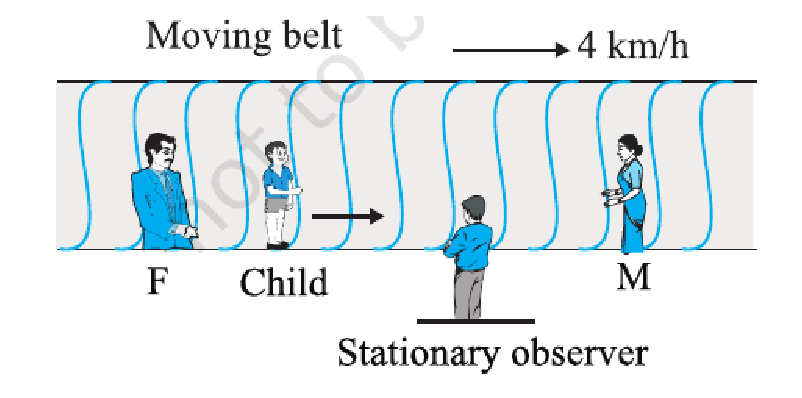
\includegraphics[width=\columnwidth]{./figs/11-1-3-26.eps}
\caption{}
\label{fig:3.26}
\end{figure}

\item A constant retarding force of 50 N is applied to a body of mass 20 kg moving initially with a speed of 15 $m s^{-1}$
. How long does the body take to stop ?
\item  A constant force acting on a body of mass 3.0 kg changes its speed from 2.0 $m s^{-1}$ to 3.5 $m s^{-1}$
in 25 s. The direction of the motion of the body remains unchanged. What is the magnitude and direction of the force ?
\item  A body of mass 5 kg is acted upon by two perpendicular forces 8 N and 6 N. Give the magnitude and direction of the acceleration of the body.
\item  The driver of a three-wheeler moving with a speed of 36 km/h sees a child standing in the middle of the road and brings his vehicle to rest in 4.0 s just in time to save the child. What is the average retarding force on the vehicle ? The mass of the three-wheeler is 400 kg and the mass of the driver is 65 kg.
\item  A rocket with a lift-off mass 20,000 kg is blasted upwards with an initial acceleration of 5.0 $m s^{-2}$. Calculate the initial thrust (force) of the blast.
\item A man of mass 70 kg stands on a weighing scale in a lift which is moving 
\begin{enumerate}
\item upwards with a uniform speed of 10 $m s^{-1}$
,
\item downwards with a uniform acceleration of 5 $m s^{-2}$ 
\item  upwards with a uniform acceleration of 5 $m s^{-2}$ 
What would be the readings on the scale in each case?
\item What would be the reading if the lift mechanism failed and it hurtled down freely under gravity ?
\end{enumerate}
\item Two bodies of masses 10 kg and 20 kg respectively kept on a smooth, horizontal surface are tied to the ends of a light string. A horizontal force F = 600 N is applied to 
\begin{enumerate}
\item A, 
\item B 
\end{enumerate}
along the direction of string. What is the tension in the string in each case?
\item Two masses 8 kg and 12 kg are connected at the two ends of a light inextensible string that goes over a frictionless pulley. Find the acceleration of the masses, and the tension in the string when the masses are released.
\item Two billiard balls each of mass 0.05 kg moving in opposite directions with speed 6 $m s^{-1}$ collide and rebound with the same speed. What is the impulse imparted to each ball due to the other ?
\item  A shell of mass 0.020 kg is fired by a gun of mass 100 kg. If the muzzle speed of the shell is 80 $m s^{-1}$
, what is the recoil speed of the gun ?
\item Figure \ref{fig:5.18} shows a man standing stationary with respect to a horizontal conveyor belt that is accelerating with 1 $m s^{-2}$
. What is the net force on the man? If the
coefficient of static friction between the man's shoes and the belt is 0.2, up to what acceleration of the belt can the man continue to be stationary relative to the belt ? (Mass of the man = 65 kg.)
\begin{figure}[!ht]
\centering
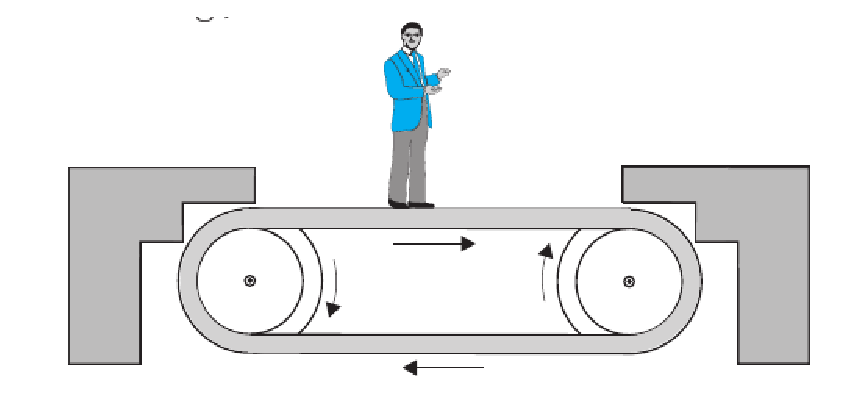
\includegraphics[width=\columnwidth]{./figs/11-1/5/5.18.eps}
\caption{}
\label{fig:5.18}
\end{figure} 

\item  A stream of water flowing horizontally with a speed of 15 $m s^{-1}$ gushes out of a tube of
cross-sectional area 10$^{-2} m^2$, and hits a vertical wall nearby. What is the force exerted on the wall by the impact of water, assuming it does not rebound ?
\item Ten one-rupee coins are put on top of each other on a table. Each coin has a mass $m$. Give the magnitude and direction of 
\begin{enumerate}
\item the force on the 7th coin (counted from the bottom) due to all the coins on its top,
\item the force on the 7th coin by the 8th coin,
\item  the reaction of the 6th coin on the 7th coin.
\end{enumerate}
\item  A block of mass 25 kg is raised by a 50 kg man in two different ways as shown in Fig. \ref{fig:5.19}. What is the action on the floor by the man in the two cases ? If the floor yields to a normal force of 700 N, which mode should the man adopt to lift the block without the floor yielding ?
\begin{figure}[!ht]
\centering
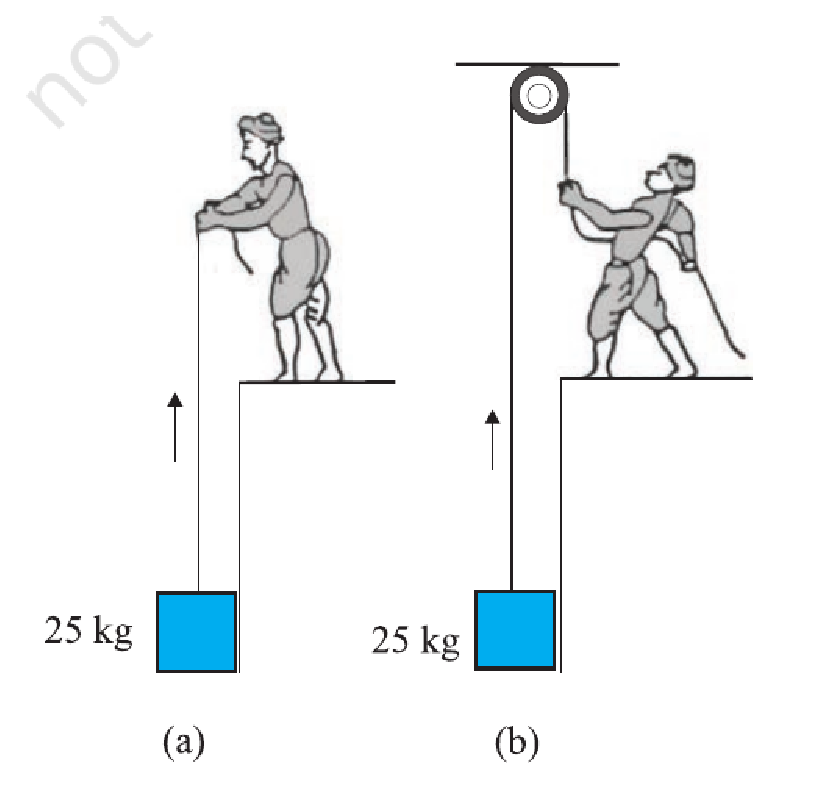
\includegraphics[width=\columnwidth]{./figs/11-1/5/5.19.eps}
\caption{}
\label{fig:5.19}
\end{figure} 

coin (counted from the bottom) due to all the coins on its top, coin by the eighth coin,
\item A monkey of mass 40 kg climbs on a rope (Fig. \ref{fig:5.20}) which can stand a maximum tension of 600 N. In which of the
following cases will the rope break: the monkey 
\begin{enumerate}
\item climbs up with an acceleration of 6 $m s^{-2}$ 
\item climbs down with an acceleration of 4 $m s^{-2}$ 
\item  climbs up with a uniform speed of 5 $m s^{-1}$
\item  falls down the rope nearly freely under gravity?
\end{enumerate}
\begin{figure}[!ht]
\centering
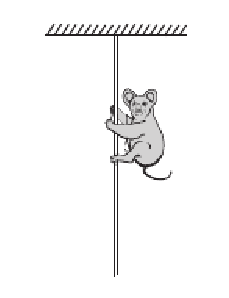
\includegraphics[width=\columnwidth]{./figs/11-1/5/5.20.eps}
\caption{}
\label{fig:5.20}
\end{figure} 

\item Two bodies A and B of masses 5 kg and 10 kg in contact with each other rest on a table against a rigid wall (Fig. \ref{fig:5.21}). The coefficient of friction between the bodies and the table is 0.15. A force of 200 N is applied horizontally to A. What are 
\begin{enumerate}
\item the reaction of the partition 
\item the action-reaction forces between A and B ? What happens when the wall is removed? 
\end{enumerate}
\begin{figure}[!ht]
\centering
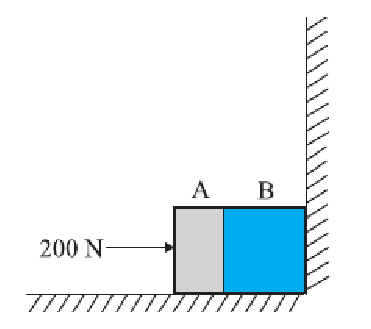
\includegraphics[width=\columnwidth]{./figs/11-1/5/5.21.eps}
\caption{}
\label{fig:5.21}
\end{figure} 
\item A block of mass 15 kg is placed on a long trolley. The coefficient of static friction between the block and the trolley is 0.18. The trolley accelerates from rest with 0.5 $m s^{-2}$
for 20 s and then moves with uniform velocity. Discuss the motion of the
block as viewed by 
\begin{enumerate}
\item a stationary observer on the ground, 
\item an observer moving with the trolley.
\end{enumerate}
\item The rear side of a truck is open and a box of 40 kg mass is placed 5 m away from the open end as shown in Fig. \ref{fig:5.22}. The coefficient of friction between the box and the surface below it is 0.15. On a straight road, the truck starts from rest and accelerates with 2 $m s^{-2}$. At what distance from the starting point Fig. \ref{fig:5.22}
does the box fall off the truck? (Ignore the size of the box).
\begin{figure}[!ht]
\centering
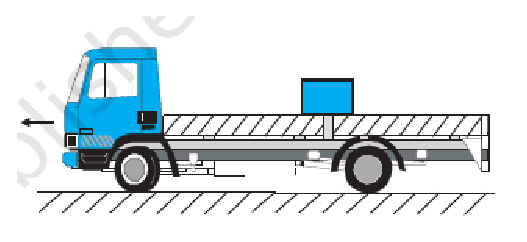
\includegraphics[width=\columnwidth]{./figs/11-1/5/5.22.eps}
\caption{}
\label{fig:5.22}
\end{figure} 
\item A body of mass 2 kg initially at rest moves under the action of an applied horizontal force of 7 N on a table with coefficient of kinetic friction = 0.1. Compute the 
\begin{enumerate}
\item  work done by the applied force in 10 s,
\item  work done by friction in 10 s, 
\item  work done by the net force on the body in 10 s,
\item  change in kinetic energy of the body in 10 s,
and interpret your results.
\end{enumerate}
\item An electron and a proton are detected in a cosmic ray experiment, the first with kinetic energy 10 keV, and the second with 100 keV. Which is faster, the electron or the proton ? Obtain the ratio of their speeds. (electron mass = $9.11 \times 10^{-31}$ kg, 
proton mass= $1.67 \times 10^{-27}$ J, 1 eV = $1.60  \times 10^{–19}$).
\item A rain drop of radius 2 mm falls from a height of 500 m above the ground. It falls with decreasing acceleration (due to viscous resistance of the air) until at half its original height, it attains its maximum (terminal) speed, and moves with uniform speed thereafter. What is the work done by the gravitational force on the drop in the first and second half of its journey ? What is the work done by the resistive force in the entire journey if its speed on reaching the ground is 10  $m s^{-1}$
\item  A molecule in a gas container hits a horizontal wall with speed 200  $m s^{-1}$ and angle 30\degree
with the normal, and rebounds with the same speed. Is momentum conserved in the collision ? Is the collision elastic or inelastic ?
\item A pump on the ground floor of a building can pump up water to fill a tank of volume 30 $m^3$ in 15 min. If the tank is 40 m above the ground, and the efficiency of the pump is 30\%, how much electric power is consumed by the pump ?
\item Two identical ball bearings in contact with each other and resting on a frictionless table are hit head-on by another ball bearing of the same mass moving initially with a speed V. If the collision is elastic, which of the following (Fig. \ref{fig:6.14}) is a possible result after collision ?
\begin{figure}[!ht]
\centering
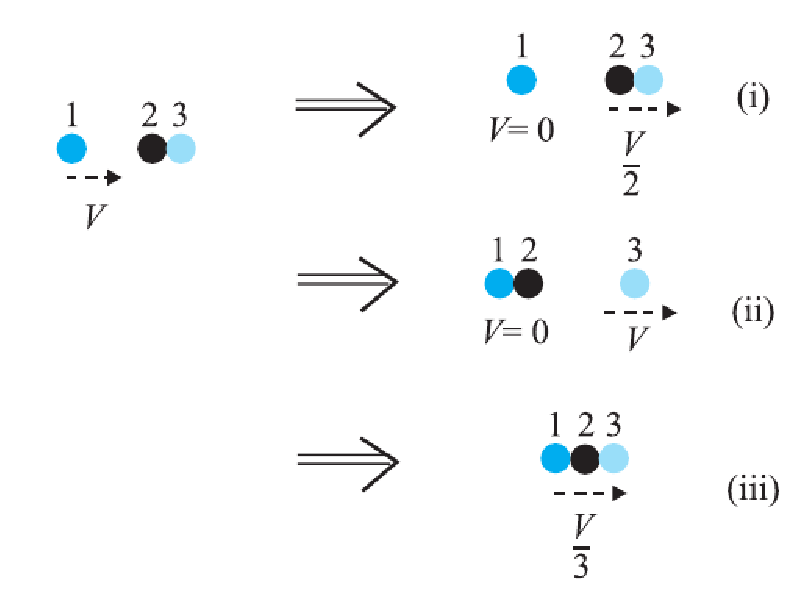
\includegraphics[width=\columnwidth]{./figs/11-1/6/6.14.eps}
\caption{}
\label{fig:6.14}
\end{figure} 
\item A trolley of mass 300 kg carrying a sandbag of 25 kg is moving uniformly with a speed of 27 km/h on a frictionless track. After a while, sand starts leaking out of a hole on the floor of the trolley at the rate of 0.05 $kg s^{-1}$. What is the speed of the trolley after the entire sand bag is empty ?
\item A person trying to lose weight (dieter) lifts a 10 kg mass, one thousand times, to a height of 0.5 m each time. Assume that the potential energy lost each time she lowers the mass is dissipated. 
\begin{enumerate}[label=(\alph*)]
\item  How much work does she do against the gravitational force ? 
\item  Fat supplies $3.8 \times 10^7J$ of energy per kilogram which is converted to mechanical energy with a 20\% efficiency rate. How much fat will the dieter use up?
\end{enumerate}
\item A family uses 8 kW of power. 
\begin{enumerate}[label=(\alph*)]
\item  Direct solar energy is incident on the horizontal surface at an average rate of 200 W per square meter. If 20\% of this energy can be converted to useful electrical energy, how large an area is needed to supply 8 kW? 
\item  Compare this area to that of the roof of a typical house.
\end{enumerate}
\item A bolt of mass 0.3 kg falls from the ceiling of an elevator moving down with an uniform speed of 7 $m s^{-1}$
. It hits the floor of the elevator (length of the elevator = 3 m) and does
not rebound. What is the heat produced by the impact ? Would your answer be different if the elevator were stationary ?
\item  A trolley of mass 200 kg moves with a uniform speed of 36 km/h on a frictionless track. A child of mass 20 kg runs on the trolley from one end to the other (10 m away) with a speed of 4 $m s^{-1}$
relative to the trolley in a direction opposite to the its motion, and
jumps out of the trolley. What is the final speed of the trolley ? How much has the trolley moved from the time the child begins to run ?
\item The angular speed of a motor wheel is increased from 1200 rpm to 3120 rpm in 16 seconds. 
\begin{enumerate}[label=(\alph*)]
\item  What is its angular acceleration, assuming the acceleration to be uniform? 
\item  How many revolutions does the engine make during this time?
\end{enumerate}
\item The planet Mars has two moons, phobos and delmos. 
\begin{enumerate}[label=(\alph*)]

\item  phobos has a period 7 hours, 39 minutes and an orbital radius of 9.4 $\times$103
km. Calculate the mass
of mars. 
\item  Assume that earth and mars move in circular orbits around the sun, with the martian orbit being 1.52 times the orbital radius of the earth. What is the length of the martian year in days ?
\end{enumerate}
\item Given $k = 10^{-13} s^2 m–3 $
. The moon is at a distance of 3.84 $\times$ 105 km from the earth. Obtain its
time-period of revolution in days.
\item You are given the following data: $g = 9.81 ms^{–2}, R_E = 6.37 \times 106
 m$, the distance to the moon $R = 3.84 \times 108 m$  and the time period of the 
moon’s revolution is 27.3 days. Calculate the mass of the earth $M_E$ in two different ways.
\item A 400 kg satellite is in a circular orbit of radius $2R_E$
about the Earth. How much
energy is required to transfer it to a circular orbit of radius $4R_E$
? What are the changes in the kinetic and potential energies ?
\item Io, one of the satellites of Jupiter, has an orbital period of 1.769 days and the radius of the orbit is 4.22 $\times$ 108
m. Show that the mass of Jupiter is about one-thousandth that of the sun.
\item  Let us assume that our galaxy consists of 2.5 $\times 10^{11}$ stars each of one solar mass. How 
long will a star at a distance of 50,000 ly from the galactic centre take to complete one revolution ? Take the diameter of the Milky Way to be 105 ly.
\item A rocket is fired from the earth towards the sun. At what distance from the earth’s centre is the gravitational force on the rocket zero ? Mass of the sun = 2$\times 10^{30}$ kg,
mass of the earth = 6$\times 10^{24}$.  Neglect the effect of other planets etc.  (Orbital radius =  1.5 $\times 10^{11}$
m).
8.13 How will you 'weigh the sun', that is estimate its mass? The mean orbital radius of the earth around the sun is 1.5 $\times 10^8$
km.
\item A saturn year is 29.5 times the earth year. How far is the saturn from the sun if the earth is 1.50 $\times 10^8$ km away from the sun ?
\item  A body weighs 63 N on the surface of the earth. What is the gravitational force on it due to the earth at a height equal to half the radius of the earth ?
\item Assuming the earth to be a sphere of uniform mass density, how much would a body weigh half way down to the centre of the earth if it weighed 250 N on the surface ?
\item A rocket is fired vertically with a speed of 5 $km s^{-1}$. How far
from the earth does the rocket go before returning to the earth ?  Mass of the earth = $6.0 \times 10^{24}$ kg.
kg; mean radius of the earth = $6.4 \times 106 m; G = 6.67 \times 10^{-11} N m^2 kg^{–2}$. 
\item  The escape speed of a projectile on the earth’s surface is 11.2 $km s^{-1}$ from the earth's surface. A body is
projected out with thrice this speed. What is the speed of the body far away from the earth? Ignore the presence of the sun and other planets.
\item  A satellite orbits the earth at a height of 400 km above the surface. How much energy must be expended to rocket the satellite out of the earth's gravitational influence? Mass of the satellite = 200 kg; mass of the earth = $6.0\times 10^{24} kg$ radius of 
the earth = $6.4 \times 10^6$ m; $G = 6.67 \times 10^{-11} N m^2$
\item Two stars each of one solar mass (= $2\times10^{30}$ kg) are approaching each other for a head on collision. When they are a distance $10^9$ km, their speeds are negligible. What is
the speed with which they collide ? The radius of each star is $10^4$ km. Assume the stars to remain undistorted until they collide. (Use the known value of G).

\item  Two heavy spheres each of mass 100 kg and radius 0.10 m are placed 1.0 m apart on a horizontal table. What is the gravitational force and potential at the mid point of the line joining the centres of the spheres ? Is an object placed at that point in equilibrium? If so, is the equilibrium stable or unstable ?
\item As you have learnt in the text, a geostationary satellite orbits the earth at a height of nearly 36,000 km from the surface of the earth. What is the potential due to earth's gravity at the site of this satellite ? (Take the potential energy at infinity to be zero). Mass of the earth = $6.0\times10^{24}$
kg, radius = 6400 km.
\item  A star 2.5 times the mass of the sun and collapsed to a size of 12 km rotates with a speed of 1.2 rev. per second. (Extremely compact stars of this kind are known as neutron stars. Certain stellar objects called pulsars belong to this category). Will an object placed on its equator remain stuck to its surface due to gravity ? (mass of the sun = $2\times10^{30}$
kg).
\item  A spaceship is stationed on Mars. How much energy must be expended on the spaceship to launch it out of the solar system ? Mass of the space ship = 1000 kg; mass of the sun = $2\times10^{30}$
kg; mass of mars = $6.4\times10^{23}$ radius of mars = 3395 km; radius of the orbit of mars = $2.28 \times10^8$ km; $G = 6.67\times10^{-11} N m^2$. 
\item A rocket is fired 'vertically' from the surface of mars with a speed of 2 $km s^{-1}$. If 20\%
of its initial energy is lost due to martian atmospheric resistance, how far will the rocket go from the surface of mars before returning to it ? Mass of mars = $6.4\times10^{23}$
kg; radius of mars = 3395 km; $G = 6.67\times10^{-11} N m^2 kg^{–2}$.
\end{enumerate}
